\begin{figure}[t]
    \centering
    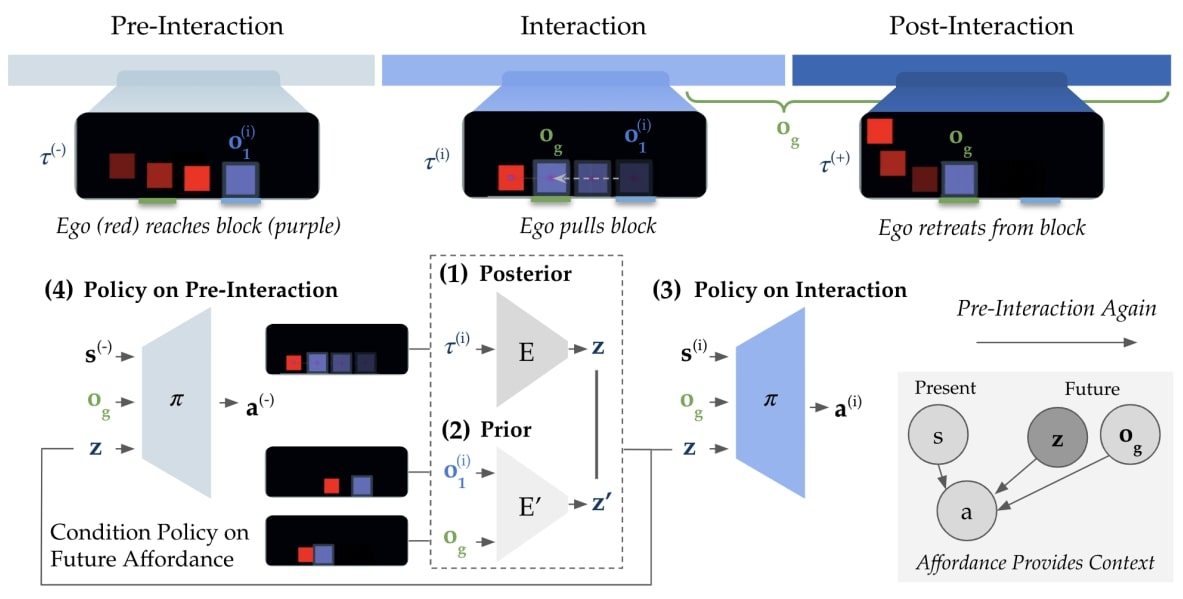
\includegraphics[width=0.7\textwidth]{figures/images/plato/plato.jpg}
    \caption{PLATO architecture proposed in \cite{belkhale2023plato}. The architecture is composed of different stages. (1) The posterior encoder \( E \) encodes the interaction sequence \( \tau^{(i)} \) into the affordance \( z \). (2) The prior encoder \( E' \) encodes the object initial state \( o^{(i)}_1 \) and goal state \( o_g \) to predict \( z \), with \( o_g \) sampled after the interaction. (3) The policy is trained to output actions during the interaction period conditioned on the affordance. Simultaneously, (4) it is trained to output actions during the pre-interaction period conditioned on the ``future" affordance.
    }
    \label{fig:plato}
    
\end{figure}

\begin{figure}[t]
    \centering
    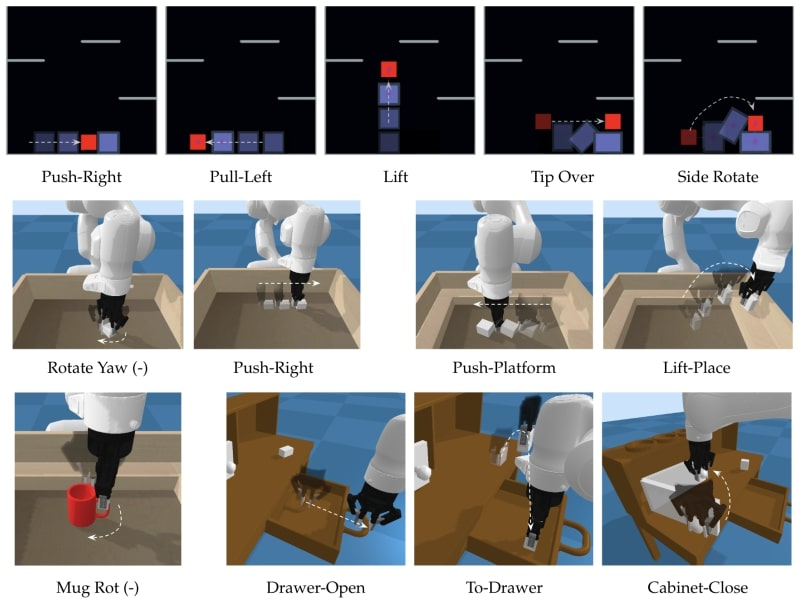
\includegraphics[width=0.7\textwidth]{figures/images/plato/tasks.jpg}
    \caption{ Testing scenarios and primitives proposed in \cite{belkhale2023plato}. (Top) \textbf{Block2D} Environment primitive examples. (Center) \textbf{Block3D} and \textbf{Block3DPlatform} primitive examples. (Bottom) The left image shows an example primitive in \textbf{Mug3D-Platforms}. The right three images show sample tasks from \textbf{Playroom3D}.}
    \label{fig:plato_task}
    
\end{figure}